%!TEX root=thesis.tex

\chapter{Radio Cross-identification}
\label{cha:passive-learning}
  % In this chapter I'll talk about a machine learning approach to the cross-identification problem (i.e. my pipeline).

  In this chapter, I develop a machine learning approach to the radio cross-identification problem. First, I will discuss different ways to train and use a classifier for the task, in particular framing the cross-identification problem as an object localisation problem. Then, I will discuss the available training data and how I chose to process it. Finally, I will present results against a dataset of expert labels, and compare these results to those found by other methods.

\section{Cross-identification as Binary Classification}
\label{sec:framing-as-classification}
  
  Given a radio object, we want to locate the host galaxy containing the AGN emitting that object. In general, there may be multiple hosts associated with one radio object (such as in Figure \ref{fig:two-hosts}), but we make the assumption that there is only one. This is the same assumption made by Radio Galaxy Zoo \todo{cite:rgz-analysis-github(?)}.

  \begin{figure}[!ht]
    \centering
    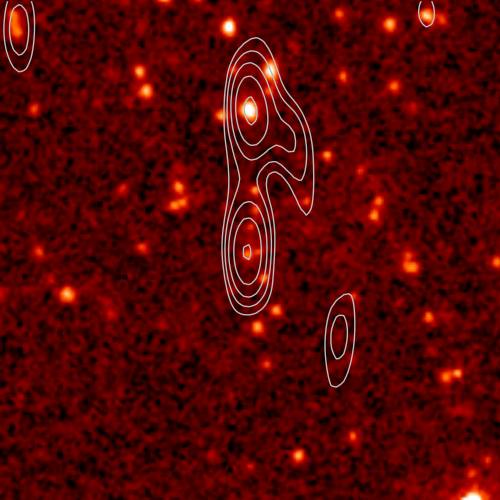
\includegraphics[width=0.5\textwidth]{images/CI0370C1_heatmap+contours.png}
    \caption{A radio object (ARG0003ra1) with two host galaxies. This radio
      object is actually two radio objects that have been incorrectly detected
      as one, and there is one host galaxy for each object.}
    \label{fig:two-hosts}
  \end{figure}

  We can interpret this as an object localisation problem. As input, we have an
  image of the radio sky, and we want to locate a host galaxy in this image. A
  common way to find an object in an image is by using a sliding window. A
  fixed-size image patch centred on each pixel is taken as a feature
  representation of that pixel. This is then used as input to a classification
  model which outputs a probability for each pixel, with higher probabilities
  corresponding to higher likelihood of the object being located at that pixel.
  The pixel with the highest rating is considered the location of the object.
  This approach can be improved by intelligently selecting candidate pixels and
  only testing these. For the cross-identification problem, we can use galaxy
  locations as candidate pixels, with galaxies found in infrared surveys such
  as WISE and SWIRE. Additionally, astronomical measurements such as flux may be taken as additional features for each candidate pixel, giving more information to the classifier.

  This approach can be formalised as follows. Consider a set $\mathcal X$ of
  candidate host galaxies, and a radio object $r$ that we want to assign a
  host galaxy. Let $y : \mathcal X \to \{0, 1\}$ represent whether a given $x
  \in \mathcal X$ is the host galaxy associated with $r$. If we assume that a
  radio object has exactly one associated host galaxy, then there exists
  exactly one $x \in \mathcal X$ such that $y(x) = 1$, and for all other $x \in
  \mathcal X$, $y(x) = 0$. The cross-identification task then amounts to
  modelling $p(y(x) = 1 \mid x, r)$. Once this distribution is modelled, the
  host galaxy associated with $r$ is given by
  \begin{equation}
      \label{eq:cross-identification}
      \mbox{host}(r) = \underset{x}{\mbox{argmax}}\ p(y(x) = 1 \mid x, r).
  \end{equation}

  Ideally, $\mathcal X$ is the set of all galaxies. This is clearly
  intractable, so as an approximation we use a catalogue of infrared objects
  near the radio object of interest, taken from an infrared survey. We also
  make the assumption that the host galaxy is within $1'$ of the radio object
  --- while this doesn't hold in general, systems larger than $1'$ are rare and
  require human insight to discover \citep{banfield16}.

\section{Data Sources}
\label{sec:data}

  To learn the cross-identification distribution (Equation \ref{eq:cross-identification}), we need a set of radio objects, a set of candidate host galaxies, and a set of existing cross-identifications for training. I have chosen to use the ATLAS radio survey for radio objects and the WISE survey for candidate host galaxies. The training cross-identifications are based on the Radio Galaxy Zoo.

  \subsection{Radio Data}
  \label{ssec:radio-data}

    The ATLAS survey \citep{franzen15} \todo{talk about this in the astro chapter} provides both a catalogue of detected radio objects and a radio image of the CDFS and ELAIS-S1 fields.

    \begin{figure}[!ht]
      \centering
      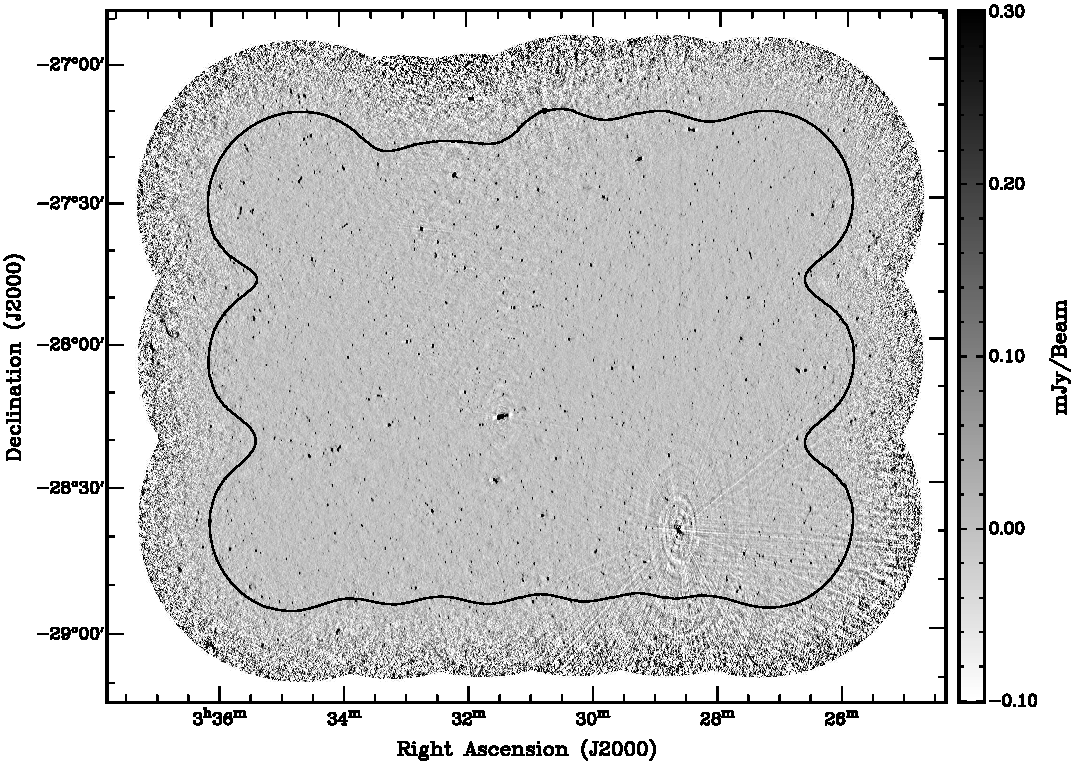
\includegraphics[width=0.8\linewidth,]{images/ATLAS-CDFS-cropped.pdf}
      \caption{ATLAS observations of CDFS. Reproduced from \citet{franzen15}.}.
      \label{fig:cdfs}
    \end{figure}

    The catalogue contains around 2400 objects in the CDFS field, all of which have been labelled by expert astronomers \citep{norris06}, by prior algorithms for automated cross-identification \citep{fan15}, and by Radio Galaxy Zoo volunteers \citep{banfield15}. The ELAIS-S1 field does not have Radio Galaxy Zoo classifications as it was not included by the Radio Galaxy Zoo researchers. The existence of expert, algorithmic, and crowdsourced labels makes ATLAS-CDFS an excellent set of radio objects for developing and testing machine learning approaches to cross-identification. Additionally, ATLAS is considered a pilot for the upcoming Evolutionary Map of the Universe survey, which will provide the majority of radio objects needing cross-identification in the future \citep{banfield15}.

    \todo{talk about ATLAS image in the astro chapter}

    The catalogue contains the name and position of each radio object, as well as various metadata such as the noise level and the flux. I have chosen to ignore the metadata and only use the position information. The positions are used to extract a $5' \times 5'$ from the full ATLAS image of the CDFS field, centred on each radio object. These image patches represent the radio object in the object localisation problem.

  \subsection{Infrared Data}

    Both the SWIRE and WISE surveys have imaged the CDFS field in infrared wavelengths. Of these, WISE is more commonly used, so I have chosen to use WISE as a source of candidate host galaxies. Like ATLAS, WISE provides both a catalogue of detected objects as well as images.

    The WISE catalogue contains names, positions, and astronomical measurements for all detected infrared objects. I used the positions to generate features for each candidate host, and the raw flux measurements as additional features. Feature generation is described in Section \ref{sec:features}. I chose to use the fluxes as they have the most physical meaning \todo{citation needed}.

    I have chosen to not use image data from WISE. Preliminary experiments showed that there was not much information gained from the use of infrared images, and using infrared images made the classifier more complex. Future work may use infrared images to improve the classifier.

  \subsection{Radio Galaxy Zoo Consensus Labels}
  \label{sec:consensuses}

    \todo{move lots of this to the astro section}
    
    Radio Galaxy Zoo volunteers are first asked to select combinations of radio
    objects that correspond to one radio source, and are then asked to select
    the location of the corresponding host galaxy \citep{banfield15}. Each
    radio subject is labelled by multiple volunteers. These labels are then
    collated as follows. First, the most common combination of radio objects is
    selected, and all labels that have a different combination are discarded.
    This radio combination is called the consensus radio combination. Then, the
    density of host location labels is estimated using Gaussian kernel density
    estimation (KDE), and the highest density location is selected. This is
    called the consensus host location. The consensus host location is then
    matched to the nearest infrared object.

    An alternative way to find the consensus host location is by using a
    clustering algorithm such as $k$-means. Host locations are clustered and
    the cluster containing the most locations is taken to represent the
    consensus; the consensus location is then the mean of the cluster. This is
    faster and more robust than using KDE, but requires $k$ to be known. $k$
    can be estimated using an algorithm such as PG-means \citep{hamerly07} or by
    choosing $k$ to minimise some information criterion \todo{cite:sklearn}.
    The consensus labels for the data associated with this thesis were found in
    this way, fitting a Gaussian mixture model to the host locations with the
    number of Gaussians chosen to minimise the Bayesian information criterion.

    Repeated volunteer labelling helps to reduce noise in the labels. This is
    necessary as the volunteers are not experts, and may incorrectly label the
    subject. The hope is that the majority of volunteers will correctly label
    subjects, which seems to be the case for radio subjects where more than
    75\% of volunteers agree \citep{banfield15}. The number of times a radio
    subject is shown to different volunteers is called the redundancy. The
    redundancy is 5 if the subject is a compact source, and 20 for all other
    sources. These numbers were chosen based on the redundancy levels of the
    original Galaxy Zoo project [Banfield, personal communication] \todo{Is
    this how to cite personal communication? Alternatively, is this written
    down somewhere?}. Since labels with radio combinations that disagree with
    the consensus are discarded, the redundancy is usually lower in practice
    when finding the host location. This can lead to very low redundancy input
    to KDE, causing KDE to fail. This failure can usually be caught, but the
    existing solution in this case is to take the mean of all host locations.
    This is not the consensus host location in general. Another effect is that
    since more complex sources have higher levels of disagreement in the radio
    combination stage, more complex sources have more discarded volunteer
    labels, and thus lower redundancy --- so more complex sources have more
    noise in their labels.

    The training data are generated by assigning each infrared object a binary label: $0$ if the object is not associated with a radio object, and $1$ if the object is associated with a radio object.

\section{Features}
\label{sec:features}

  Each candidate potential host galaxy has an associated set of features. Some of these features are extracted from the radio image patch centred on the galaxy, and some of these features come directly from the infrared survey.

  \subsection{Astronomical Features}

  \subsection{Radio Image Features}

\section{Choosing a Binary Classifier}
\label{sec:binary-classifier}

\section{Results}
\label{sec:passive-results}
